%%
%% This is file `./samples/longsample.tex',
%% generated with the docstrip utility.
%%
%% The original source files were:
%%
%% apa7.dtx  (with options: `longsample')
%% -----------------------------------------------
%% 
%% apa7 - A LaTeX class for formatting documents in compliance with the
%% American Psychological Association's Publication Manual, 7th edition
%% 
%% Copyright (C) 2019 by Daniel A. Weiss <daniel.weiss.led at gmail.com>
%% 
%% This work may be distributed and/or modified under the
%% conditions of the LaTeX Project Public License (LPPL), either
%% version 1.3c of this license or (at your option) any later
%% version.  The latest version of this license is in the file:
%% 
%% http://www.latex-project.org/lppl.txt
%% 
%% Users may freely modify these files without permission, as long as the
%% copyright line and this statement are maintained intact.
%% 
%% This work is not endorsed by, affiliated with, or probably even known
%% by, the American Psychological Association.
%% 
%% -----------------------------------------------
%% 

% response letter for Science & Education paper: https://docs.google.com/document/d/11knIlTG488LM4kw5y8irPS8CqqBbTbdJJyGeXEFmhqY/edit

% will remove the below for submission; for reference now
% https://kubsch.shinyapps.io/Confidence_Updater
% https://github.com/MKubsch/confidence_updater

\documentclass[man, floatsintext]{apa7} % JR: for some reason, the figures aren't floating in text

\usepackage[american]{babel}
\usepackage{nicefrac}
\usepackage{todonotes}
\usepackage{epigraph}
\usepackage{amsfonts, amsmath,amssymb}
\usepackage{comment}

\newcommand{\SR}[1]{} %for EJ's bibtex file
\newcommand{\given}{\, | \,}
\newcommand{\EJ}[1]{\todo[inline, color=yellow]{  #1 }}
\newcommand{\JR}[1]{\todo[inline, color=gray]{  #1 }}
\newcommand{\MK}[1]{\todo[inline, color=red]{  #1 }}
\newcommand{\MD}[1]{\todo[inline, color=green]{  #1 }}

\usepackage{graphicx}
\graphicspath{ {images/} }

\usepackage{csquotes}
\usepackage[style=apa,sortcites=true,sorting=nyt,backend=biber, hyperref=false]{biblatex}

\usepackage{url} % This makes \url work

\DeclareLanguageMapping{american}{american-apa}
\addbibresource{bibliography.bib}
\addbibresource{referenties.bib}

\title{Why and How a Bayesian Approach Supports Science Educators and Learners to Reason Under Scientific Uncertainty}
\shorttitle{Reasoning Under Scientific Uncertainty}

\fourauthors{Joshua M. Rosenberg}{Marcus Kubsch}{Eric-Jan Wagenmakers}{Mine Dogucu}
\fouraffiliations{University of Tennessee, Knoxville}{IPN - Leibniz Institute for Science and Mathematics Education}{University of Amsterdam}{University of California, Irvine}

\leftheader{Weiss}

\abstract{
Uncertainty is ubiquitous in science, but scientific knowledge is often represented to the public and in educational contexts as certain and immutable. This contrast can foster distrust when scientific knowledge develops in ways that can be perceived as reversals, e.g., consider changing recommendations regarding mask wearing during the COVID pandemic. Adding to this issue is that when scientists try to communicate their uncertainty, research has demonstrated that many people--learners and experts alike--struggle to interpret the statistics that are used to make draw inferences from scientific data. We argue that a Bayesian perspective can offer a coherent, holistic solution to these problems. Central to a Bayesian approach to teaching, learning, and sense-making is viewing uncertainty \ital{probabilistically}, as doing so provides a language for expressing the degree of beliefs about what is known about the world. In this paper, we describe prior research on uncertainty and probability in science (and science education) and review how people learn about these ideas. Then, we provide a primer on Bayes' Theorem and discuss general principles relevant to science education that follow from Bayes' Theorem. Finally, we focus on \ital{how} to make Bayesian approaches to reasoning about uncertainty practical for science educators through the introduction of an interactive, accessible tool. We conclude with a call for future research to use a Bayesian perspective to bolster trust in science and to provide a coherent frame for considering  uncertainty in data and evidence within and beyond science classrooms.
}

\keywords{Bayesian, uncertainty, probability, trustworthiness, statistics}

\authornote{
   \addORCIDlink{Joshua M. Rosenberg}{0000-0003-2170-0447}
   \addORCIDlink{Marcus Kubsch}{0000-0001-5497-8336}
   \addORCIDlink{Eric-Jan Wagenmakers}{0000-0003-1596-1034} 
   \addORCIDlink{Mine Dogucu}{0000-0002-8007-934X}
   \\
   Joshua M. Rosenberg and Marcus Kubsch contributed equally to this manuscript.
}

\begin{document}

\maketitle

Uncertainty is ubiquitous in science. Consider, for instance, uncertainty due to measurement error or temporal variability in the characteristics under study.  \parencite{fuller2009measurement}. Another form of uncertainty is its central role within explanatory theories--such as those associated with evolution and quantum physics--for which models take the form of probabilistic statements about the world \parencite{g00}. 

Negotiating the many forms of uncertainty through constructively arguing--and building toward consensus at the same time that uncertainty is present--is a key part of the scientific process \parencite{g00}. It is also a key part of science education \parencite{duschl2008science, t00, nrc12, manz2018supporting, so12, n11}. Concomitantly, some philosophers of science have suggested that science is a process that builds increasingly better models which allows us to make increasingly more accurate predictions \parencite{g10,  n02, r77, lakatos1976falsification, feyerabend1993against, carnap1935philosophy, Kuhn1962}. \\

However, while scientists, historians, and philosophers of science are well aware of the uncertainty and limitations around uncertain scientific knowledge and negotiating and arguing from evidence \parencite{polanyi1962tacit, polanyi1966logic}, scientific knowledge is often represented to the public and in educational contexts as certain and immutable \parencite{d90, manz2018supporting, carey1993understanding}. Trust in science can erode and has eroded when scientists individually or collectively change their views, such as during the first phase of the COVID-19 crisis, when scientists faced serious criticism from the public, the media, and elected representatives for changing their recommendations based upon new scientific data and findings \parencite[]{vanderbleseffects2020,kreps_model_2020}. A similar tension between how certain scientific knowledge is perceived and how uncertain it really is concerns vaccines for COVID-19--a tension that involves reconciling robust but still initial clinical trial data and new data from population-level vaccination efforts. This tension also involves regulatory organizations, politicians, and medical, pharmaceutical, and scientific experts making policy-level recommendations (and individual decisions) amid uncertainty \parencite[]{vanderbleseffects2020, kreps_model_2020}. \\

In this paper, we argue that these challenges concerning trust in scientific knowledge can be addressed by considering scientific knowledge not as correct or incorrect or true or false, but rather to consider the degrees of belief that one might express in light of prior information and new evidence. In other words, we argue for the use of a Bayesian perspective that emphasizes \ital{subjective probability} \parencite[]{batanero2016research,, konold1991understanding}. Particularly, we argue that some of the challenges around trust in science can begin to be addressed by taking a Bayesian perspective to how people--and students--understand uncertainty. Thus, this paper is \ital{not} about how scientists, statisticians might use Bayesian methods; books address this topic \parencite[]{gelman1995bayesian, Kruschke2015Book}, and papers now exist on how educational researchers can use such methods \parencite{kubsch2021beyond, levy2016advances}. Instead, we claim that \ital{science learners} can use Bayesian reasoning to be able to reason about uncertainty in a more principled and flexible manner. We make this argument by drawing on research from the work of individuals from diverse disciplines: a) psychologists using Bayesian models of cognition \parencite{g12, tgk06}, b) statisticians and statistics educators advancing tools and practices for Bayesian methods \parencite{a02, b02, h_a20, h_j20,me14, s07} and c) science education scholars who have advanced a Bayesian perspective on argumentation \parencite{n11, s07} and scientific reasoning \parencite{warren_quantitative_2018,warren_impact_2020}. In doing so, we claim that Bayes' Theorem does not only have use as a mathematical or statistical tool, but also that Bayesian reasoning can provide an intuitive way for people to think about data and evidence under uncertainty \parencite{g12} and in classroom contexts \parencite{ll20, n11, s07, so12, w17, warren_impact_2020}. \\

As this introduction has suggested, central to the contributions of Bayesian methods is viewing uncertainty \ital{probabilistically}, as probabilities can provide a language for expressing the degree of uncertainty in our knowledge in a wide range of domains \parencite{g12}, as we discuss next. \\

\section{Uncertainty in Science}

Probability and uncertainty are ubiquitous in scientific methodologies, scientific concepts, and in how science is communicated \parencite{gsoobmc17}. The practice of science often begins with \ital{measurement}, which has a random component \parencite{fuller2009measurement} that arises from random variations in the measurement process. Measurement error limits the certainty that one can have in the measurements and reducing that measurement error has been critical for many discoveries in science, such as the sorting out of the periodic table that has resulted in the representation as it is known today \parencite{fco15}. Deciding on adequate statistical procedures to determine measurement uncertainty is not always easy and it regularly sparks debate, e.g., consider a recent study on the relationship between SARS-CoV-2 viral load and patient age by \textcite{jmvbzhd20} that was heavily debated in the scientific community \parencite{frick_peer-review_2020} because the authors initially discretized a continuous variable, reducing statistical power. \\

Probability and uncertainty are not only integral to some science practices (such as analyzing and interpreting data; see \textcite[]{nrc12}) but are also a part of explanatory models of and theories for scientific concepts. For example, in the context of Heisenberg’s uncertainty principle--more generally in quantum mechanics \parencite{feynman1951operator}--confidence is limited not only by measurement error but in principle--even in the perfect experimental setup, there is no deterministic outcome. Instead, one has to calculate the probability of each possible outcome using the Born rule. To this day, there is an ongoing argument about how to interpret the puzzling quantum mechanical phenomena such as quantum tunneling \parencite{c19}. \\

Another example of how probability and uncertainty are central to scientific concepts and respective learning activities is evolution \parencite{fsnh19}. Evolution is modeled as a probabilistic process as the emergence of new variations (e.g., through mutations) can only be described probabilistically. Further, the continued survival of these variations with the population is governed by phenomena such as natural selection or random drift which also escape a deterministic description and are thus modeled probabilistically. Similar to quantum physics, how to interpret this probability has also sparked debate among researchers \parencite{m16}. \\

Given that probability and uncertainty spark and sustain debate among scientists, it is perhaps unsurprising that misinterpretations happen when scientists in the natural and engineering sciences communicate about their findings with their peers or the public \parencite[]{gkv04, c14, mg17}. For example, error bars in the form of confidence intervals are routinely interpreted as distributions that assign a higher probability to the center of the interval \parencite{kl18}. Another example concerns very low \ital{p}-values, which are sometimes misinterpreted as effect sizes \parencite{gc17, n14} although \ital{p}-values describe how \ital{incompatible} a set of data is with a set of assumptions). Futher, p-values and Null-Hypothesis Significance Testing (NHST) have been criticized for fostering black or white thinking: either accept or reject the null hypothesis, leaving little room for uncertainty even when there is \parencite[]{cohen_earth_1994,aczel_quantifying_2017}. 

In short, misunderstandings of statements about probability and uncertainty are common across the range of modes in which scientists communicate about their work--and these can lead to misinterpretations that can diminish trust in science and the process through which scientific knowledge is constructed \parencite{vanderbleseffects2020,kreps_model_2020}. \\

We next discuss the role of uncertainty not in science, but in science education contexts. \\

\section{Uncertainty in Science Education}

\subsection{The Roles of Probability Across Scientific Disciplines}


Probability and chance events play an important role in the life sciences \parencite{g03, gk08}, particularly in learning about evolutionary processes \parencite{th17}, and scholars have explored how knowing about probability might impact knowledge about scientific ideas. Recently, \textcite{fsnh19} investigated the relation between statistical reasoning and acceptance and knowledge about evolution in a large sample of nearly 500 university students in the US. They found that students’ statistical reasoning capabilities are a strong predictor of both acceptance of evolution and knowledge about evolution. Research on teachers' conceptions of evolution has suggested that exposure to curricular materials that emphasized the role of randomness in evolution bolstered teachers' \ital{acceptance} of evolution, but not their understanding of it. The authors conjectured that difficulties learners face when working to understand probability and uncertainty may require extensive instruction \parencite{nadelson2010shifting}. \\

In the physical sciences, students' struggles with the probabilistic nature of quantum physics \parencite{br02} and nuclear decay \parencite{smmv17} have been established by prior research, but the underlying reasons and mechanisms remain less researched than in evolution. Research into students’ misconceptions has started to address this gap \parencite{ms15, alra14, st09}. Findings mirror the position of \textcite{bgv94}. Specifically, the concepts of probability are taught abstractly and in such a way that does not build upon the ideas that students already hold, the experiences that students have, and the language that students use. Thus, these studies affirm students' struggles with scientific concepts that are probabilistic but hint at an underlying issue of more foundational challenges with reasoning about probability beyond science education contexts. \\

Adding to this difficult state of affairs is that when scientists try to communicate their uncertainty, prior research has demonstrated that many people–learners and experts alike–struggle to interpret the statistics and derivations of statistics (such as standard errors/margins of error, confidence intervals, and p-values that establish statistical significance) and that are often used to make inferences from scientific data \parencite{gkv04, s07, tk74}. Similarly, difficulties in understanding the technical language of probability can contribute to a struggle on the part of students when learning about concepts such as evolution or nuclear decay that are modeled in terms of probabilistic statements \parencite[e.g.][]{fth17}. \\

The work of \textcite{tk74}, especially, points to a range of biases that can be elicited by the language in which statements about probability and uncertainty are framed. A prominent example is the neglect of base rate information in the (timely) context of medical testing. The probability of having a medical condition based on a positive test result is often overestimated because information about the (base) rate of people affected by the condition is not considered \parencite{kahneman_thinking_2012}; this base rate can be considered a form of prior knowledge about how probable it is that a person has a disease before considering the result of the test. The neglect of base rate information means that diagnostic tests that return positive results may not indicate that the individual truly has the disease the test is intended to detect. This also manifests itself in the prosecutor's fallacy \parencite{thompson1987interpretation}. \\

Responding to and building upon Kahneman and Tversky's work that suggests that people may not reason in a \ital{proper} (or correct) Bayesian manner, Gigerenzer and colleagues provided important insights into the underlying mechanisms for the occurrence of these biases. Their research suggests that the biases are at least partly the result of information about probability and uncertainty being provided in a way that is incompatible with the heuristics that people develop from their everyday experiences \parencite{gh95, jkg18}. Based upon this premise, \textcite{jkg18} were able to demonstrate that students judge probability significantly better when language is adopted that better aligns with the heuristics that most learners develop from their everyday experiences. In sum, it seems feasible to change representations of probability and uncertainty so that they better align with ideas and heuristics that learners hold so that they support, rather than hinder, learning. \\

Given that people struggle to understand probability, is the Bayesian account of reasoning under uncertainty a prescriptive rather than a descriptive account? We explore this question in the next section drawing on work from scholars studying children's causal reasoning under conditions of uncertainty. \\

\subsection{Bayes' Theorem and Research on How Children Learn to Reason}

In the past two decades, developmental scientists have used Bayes' Theorem to understand how children make sense of and reason about the world \parencite{g12, tgk06, tgk06, bonawitz_sticking_2019}. The notion that children (and people) weigh evidence about the world in a Bayesian way also builds upon, refines, and in some cases refutes aspects of much earlier work that documented the surprisingly complex ways that children could reason about the world \parencite{pi69}. Different from earlier work on the stages through which children develop (e.g., the work of Piaget and other developmental \ital{stage} theorists), recent work using Bayesian models considers the differences in the reasoning ability of children and adults to be a matter of degree, rather than one of kind. From contemporary views of development, children hold initial ideas and understandings that they change (or update) in ways that are concordant with how Bayes' Theorem represents the updating of an initial belief in light of data \parencite{g12}. \\

In addition to developmental research that uses Bayes' Theorem as a way to understand how children make sense of data and information in light of their initial ideas and beliefs, other, related research is also relevant. Specifically, research that studies how learners’ prior understanding influences probability judgements of different patterns in data centers on the same tension around interpreting data in light of initial beliefs that a Bayesian perspective highlights \parencite[e.g., ][]{kd88, mkm07, ssc07}. For example, the work of \textcite{kd88} considers the scientific reasoning process in terms of the two “searches” people undertake, of their beliefs and hypotheses in their mind and data and evidence collected or analyzed as a part of some investigation. Scientific reasoning involves the coordination of these two “problem” spaces, but neither entirely outweighs the other, in a manner similar to the Bayesian process of updating initial beliefs in light of data. We know that people--even children--can and do update their beliefs in light of data, though the extent to which they do depends on many factors, including how much people \ital{could} know about the topic to begin with \parencite{mkk17}. \\

In addition, prior research on learners' perceptions of the plausibility of scientific explanations highlights the importance of the degrees of belief that learners hold about a particular scientific explanation \parencite[e.g., ][]{lombardi2013plausibility, lombardi2016plausibility}. This work suggests the merit of a Bayesian perspective as a potential frame or theoretical account for (in these key instances) analyzing patterns in data and conceptual change; it also has other benefits for teaching and learning. \\

Because of the advances made by research using a Bayesian perspective to understand human \ital{development} \parencite{gt07, gw12}, one might conjecture that there has been a ready application of these ideas to education. For instance, \textcite{g12} wrote that the use of Bayesian methods to understand child development can serve as ``a scientific foundation for a long tradition on `inquiry-based science education''', and that adopting a Bayesian perspective ``could lead us to much more specific and scientifically supported proposals for education'' (p. 1627). However, it has largely not been the case that ``science itself could help turn young children's natural curiosity and brilliance into better science teaching and learning'' \parencite[p. 1627]{g12}, as some science education scholars have bemoaned \parencite{ls15}. Indeed, scholars have bemoaned that it is often obsolete applications of Piaget’s ideas \parencite[e.g., ][]{pi69} that represent the greatest contribution of developmental ideas to education \parencite{ls07}. \\

At the same time that opportunities to connect developmental science with science education exist, scholars have emphasized how important students' prior knowledge and understandings are to their ability to update their understanding of scientific concepts and processes \parencite[e.g., ][]{ssc07, mkm07, mkk17, ls04}--highlighting a potentially powerful connection between Bayesian methods and the priorities of science educators. Developmental and psychological research into Bayesian models of cognition supports and bolsters these educational efforts--especially science education efforts--to design instruction based around eliciting and understanding students’ ideas \parencite{gb16, hbavb20, wtbs12}. \\

Taken together, there is an opportunity to use Bayes' Theorem and Bayesian ideas to bring together and to formalize a collection of ideas that are relevant to science teaching and learning. However, a Bayesian perspective--with a few exceptions \parencite[e.g., ][]{n11, so12}--has been mostly absent from research in science education. Moreover, a Bayesian perspective may also have a role in building trust in science by representing uncertainty in a principled yet flexible way--in this way, having a potential impact on people's scientific literacy.\\

Before elaborating on the education- and science literacy-related roles for a Bayesian perspective, we introduce Bayes' Theorem from an accessible mathematical and statistical perspective (with connections to the axioms that follow from this perspective).

\section{A Primer on Bayes' Theorem}

Fundamentally, Bayes' Theorem is a mathematical procedure to understand new evidence in light of prior information. In this way, the process of updating what is already known is \ital{mathematical}, but Bayes' Theorem also includes an \ital{epistemological} component--a component related to what is known about the world. What counts as prior information should be construed very broadly--it encompasses subjective judgments of how likely an event is as well as knowledge of empirical data from other, related events. \\

The usefulness of Bayes' Theorem lies in how it presents a flexible yet principled way to update what is known in light of the evidence. Bayes' Theorem is not a cure-all; it is, instead, a formalization of something scientists and people alike do: interpret evidence in light of what is already known. It is epistemologically \ital{normative} to the extent that it is the derivation of the laws of conditional probability. \\

As represented in Equation 1, Bayes' Theorem states that at any point in time, our knowledge about the world after observing new evidence can be obtained by multiplying our prior information with something called a \emph{predictive updating factor} \parencite{RouderMorey2019,WagenmakersEtAl2016CD}:

\begin{equation*}
        \text{Posterior uncertainty} = \text{Prior uncertainty} \times \text{Predictive updating factor}
\end{equation*}

Mathematically, this can be expressed as:  
\begin{equation}
\label{eq:BayesRule}
        p(\theta \mid \text{data}) = p(\theta) \times \frac{p(\text{data} \mid \theta)}{p(\text{data})},
\end{equation}
where $\theta$ is prior information that can take the form of a  proposition, claim, hypothesis, parameter value, and any account of the world about which we are uncertain. The predictive updating factor consists of two components. First, $p(\text{data} \given \theta)$ is the \ital{likelihood}, that is, the extent to which the observed data were expected under $\theta$. Second, $p(\text{data})$ is the \ital{marginal likelihood}, that is, the extent to which the observed data were expected without conditioning on $\theta$. If the observed data are more expected (i.e., better predicted) when conditioning on $\theta$, the predictive updating factor is higher than 1, and $\theta$ becomes more credible. 

To illustrate the above equation, consider the following. The Hemlock Wooly Adelgid is an invasive insect that feeds on Eastern Hemlock trees, a tall-growing pine tree found in the Eastern United States. Because infestations can kill Eastern Hemlocks fairly rapidly (within several years), in many affected areas, people take steps to protect Eastern Hemlocks that are (or could be) affected by the Hemlock Wooly Adelgid; some systemic treatments can be effective \parencite{nps2021}. \\

A student (or a scientist) may be interested in the proportion of Eastern Hemlock trees within a specific area that exhibit signs of infection: diseased trees with visible white ``cotton ball'' clumps at the base of the needles of affected trees. Let's consider that in the location we are examining, each Eastern Hemlock tree grows about the same distance apart from every other tree (such that we may reasonably consider the distance between trees to not be a critical factor to consider in an investigation). Before beginning an analysis, we need to establish what prior information we have - the relative plausibility of the different values for the proportion of affected Eastern Hemlock trees, or $\theta$. Given what they learned in class and what they noticed walking into their school, the student's best guess may be that about half of the Eastern Hemlock trees on the playground of their school are infected. They would not be surprised if the proportion of affected trees was between 30\% and 70\%, but--based on what they learned and observed--they would be rather surprised to find either no affected trees or that all of the trees were affected. \\

This background knowledge motivates the use of the dome-shaped prior distribution shown as the dashed line in Figure~\ref{fig:WindowsMacPriorPosterior}.\footnote{This is the beta$(2,2)$ distribution.} Now suppose the student starts to collect data by observing trees on the playground of their school. The first ten observations (with \ital{Y} representing infected and \ital{N} representing not infected) are $\{Y, Y, N, Y, N, Y, Y, N, Y, N\}$: six infected trees and four not infected trees. \\

With these data in hand, we then combine our prior knowledge with the predictive updating factor and obtain the posterior distribution shown as the solid line in Figure~\ref{fig:WindowsMacPriorPosterior}. The posterior distribution is more peaked than the prior distribution, indicating that the data have sharpened our knowledge about $\theta$. In addition, the posterior distribution is higher than the prior distribution for values of $\theta$ between approximately $.4$ and $.75$: these values of $\theta$ predicted the data relatively well and have therefore gained credibility. In contrast, values of $\theta$ lower than $.4$ and higher than $.75$ predicted the data relatively poorly, which is why they have lost credibility compared to the prior.\\ 

\begin{figure*}[h]
\begin{center}
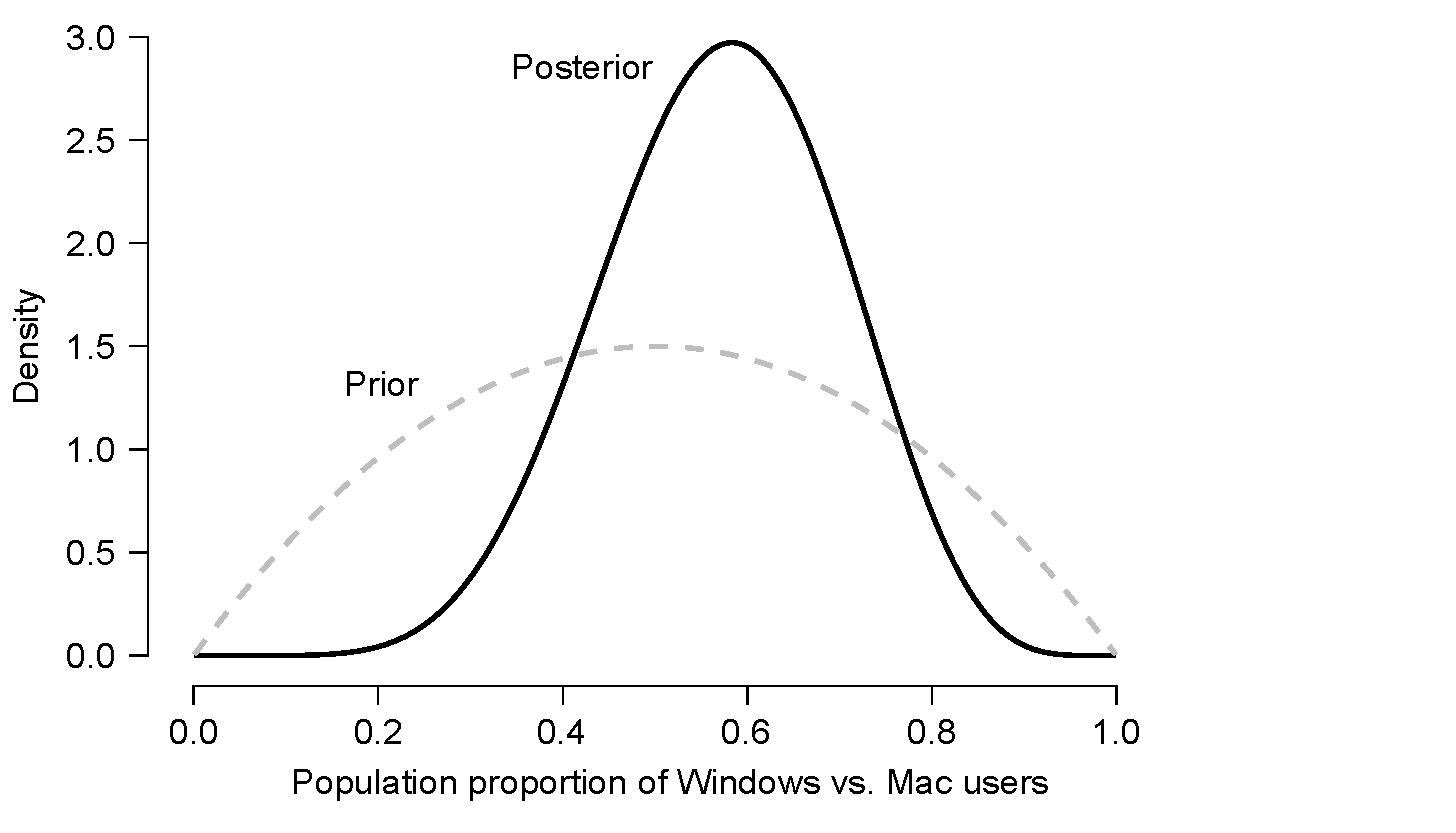
\includegraphics[width = .785\paperwidth]{WindowsMacPriorPosterior.pdf}
\caption{Example of the use of Bayes' Theorem to update prior information in light of new evidence. A dome-shaped prior distribution captures the background knowledge concerning the proportion of affected trees. Observing ten trees (six affected and four not affected) drives a knowledge update that results in a bell-shaped posterior distribution. Figure based on the \emph{Learn Bayes'} module in JASP.}
\label{fig:WindowsMacPriorPosterior}
\end{center}
\end{figure*}

Although we have demonstrated this updating process in a single step, it could also be executed sequentially, one tree at a time. For instance, the first observation we make is a $Y$, and in light of the prior, this makes the proportion of infected trees a bit higher. This slight change in knowledge is reflected in the difference between the distributions on the top two lines in Figure~\ref{fig:WindowsMacSequential}; line ``0'' represents the dome-shaped prior distribution and line ``1'' represents the posterior distribution after the first observations. Note that observing a $Y$ has nudged the distribution a little to the right. \\

Crucially, the `nudged' posterior distribution after the first observation now takes the role of the prior distribution ready to be updated by our second observation. The second observation is again a $Y$, and line ``2'' shows that the resulting posterior distribution is nudged to the right once more. At every stage in the sequential updating process, the posterior distribution based on the observations seen so far becomes the prior distribution for incorporating the information from the next observation. Specifically, the changing distributions in Figure~\ref{fig:WindowsMacSequential} show our knowledge about the world is subject to constant change, by making observations and integrating incoming information with current knowledge using Bayes' Theorem. It should be emphasized that although the updating process is conceptually different, the final outcome is identical: the shape of the posterior distribution is unaffected by whether data arrive simultaneously or sequentially. \\

\begin{figure*}[h]
\begin{center}
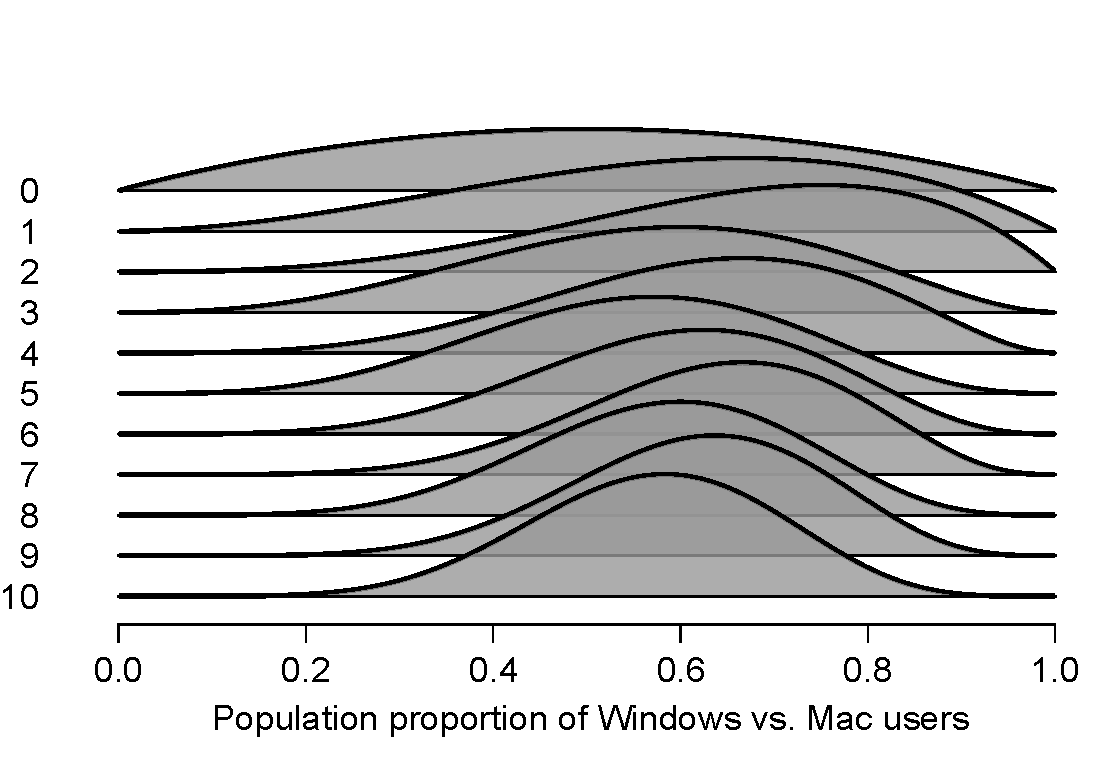
\includegraphics[width = .65\paperwidth]{WindowsMacSequential.pdf}
\caption{Updating what is known sequentially using Bayes' Theorem. A dome-shaped prior distribution (line ``0'') captures the background knowledge concerning the proportion of infected trees. Each new observation results in an update to a posterior distribution, which then becomes the prior distribution for the analysis of the next observation. Figure based on the \emph{Learn Bayes'} module in JASP.}
\label{fig:WindowsMacSequential}
\end{center}
\end{figure*}

We expand on this primer--specifically mathematical axioms that follow from Bayes' Theorem--in Appendix A.

\section{Supporting Science Learners to Navigate Uncertainty}

\subsection{The Principles That Follow From Bayes' Theorem}

As long as science instruction progresses mostly \ital{qualitatively}--our assumption for most K-12/pre-collegiate science classrooms--the features of Bayesian reasoning can help to bring a sense of coherence to the many ways in which uncertainty is manifest when students engage in scientific practices such as constructing explanations, analyzing and interpreting data, or developing and using models. \\

Thus, we argue that Bayesian reasoning can provide this coherence as its distinctive feature, through the use of ``concept of degree of belief to describe epistemic attitudes about uncertain propositions'' \parencite[, p. 2]{sprenger2019bayesian}. Such a perspective reflects an embrace of the epistemic stance that scientific knowledge is not immutable but in fact open to revision. In other words, scientific knowledge always comes attached with a degree of belief that can be updated following the rules of Bayes'’ Theorem when new evidence becomes available. The result of that updating process depends on the uncertainty of existing scientific knowledge which is then expressed in the prior. \\

In this way, Bayes' Theorem applied to the scientific process, or what we refer to as \ital{Bayesian reasoning}, emphasizes that science and scientific knowledge is always situated in context \parencite{so12} and society \parencite{driver1994constructing}. \\

These ideas about what Bayesian reasoning is can be captured in the following three principles:

\begin{enumerate}
    \item \ital{Be open to new evidence}: Scientific knowledge always comes with some uncertainty and priors that denoting absolute certainty or impossibility --by definition--prevent scientific progress. This principle expresses the Bayesian degree of belief epistemology, exemplifying that scientific knowledge is tentative and that scientists should not make absolute or certain claims. Lindley popularized this idea in statistics and coined it ``Cromwell's rule'' \parencite[p. 104]{Lindley1985}.
    \item \ital{Account for what is already known}: Evaluate new evidence in light of prior information. This emphasizes how scientific knowledge is not constructed in isolation but rather is built upon earlier information and evidence.
    \item \ital{Consider alternative explanations}: Consider the evidence in terms of compatibility with all possible outcomes; in other words, consider counterfactuals. This expresses what in Bayesian philosophy is referred to as the \ital{Simple Principle of Conditionalization} \parencite{adams1965logic}, i.e., when we weigh evidence we must consider to what extent it supports the range of possible explanations for the data. 
\end{enumerate}

Emphasizing these principles and their relations to the nature of scientific knowledge within the context of science teaching and learning can support students in connecting the frequent but often isolated references to uncertainty and limits of scientific knowledge in the Framework for K-12 Science Education \parencite{nrc12} and the NGSS \parencite{ngss2012}. The descriptions of the science practices in the \ital{Framework} \parencite{nrc12}, particularly, contain expressions such as revising models, refining explanations, critiquing arguments, and considering the limitations of the precision of the data. \\ 

However, what is lacking in these statements is an explicit and coherent rationale for why revising, refining, considering limitations is a necessary part--and in fact a feature--of science, rather than a limitation or constraint of science. Familiarizing students with the principles as core components of Bayesian reasoning can foster ideas about scientific knowledge--epistemological ideas--from which the elements of the practices that pertain to uncertainty and the limits of scientific knowledge follow naturally. Moreover, this assumption is supported by the work of \parencite{warren_impact_2020,warren_quantitative_2018} which demonstrates that integrating Bayes' reasoning into university science courses positively shifts students epistemic attitudes regarding the nature of knowing and learning. This assumption is also supported by research at the upper elementary (ages 10-11) grade levels \parencite{kazak2015bayesian, kazak2018emergent}. \\

In the following section, we provide an example of how the quantitative Bayesian updating activities in \textcite{warren_impact_2020,warren_quantitative_2018} can be made accessible to students in middle and high school by using a computational tool--specifically tailored toward students at the middle and high school grade levels (ages 12 and older). In both studies, Warren implemented Bayesian updating activities into a introductory university physics courses. The activities were added to in-class and homework tasks and generally asked students to evaluate their answers or results using Bayesian Reasoning. For example, in addition to all the usual parts of a lab report students were asked record their initial confidence in the hypothesis they would test, asked to estimate how the data they collected aligns with their initial hypothesis, and update their confidence accordingly using Bayes' theorem. In a quasi-experimental setting,  \textcite{warren_impact_2020} found that these activities positively impact students' epistemic beliefs, including beliefs regarding the nature of scientific knowledge and the presence and importance of uncertainties. \\

\subsection{Making it Practical: An Example with the Confidence Updater Widget}

\subsection{Background on the Confidence Updater Widget}

\textcite{warren_impact_2020,warren_quantitative_2018} frames the Bayesian reasoning as part of a hypothetico-deductive process \parencite[][pp. 30, 360]{popper_objective_1979}. In this process, a model is evaluated by deriving a testable hypothesis and testing it against yet unknown data. Depending on the ratio between the likelihood of observing the data if the hypothesis is true and the likelihood of observing the data if the hypothesis is false, confidence in the model decreases or increases relative to the initial confidence in the model. \\

This confidence updating can be described stating Bayes' Theorem in the following way where $\theta$ from equation (1) takes the form of a hypothesis H: 
\begin{equation}
p(H|data) = \frac{p(H)\times R}{p(H)\times R+1-p(H)}
\end{equation}

p(H|data), or our \ital{posterior}, is the confidence we can have in the hypothesis H after updating our initial confidence, or our \ital{prior}, $p(H)$ based on consideration of the \ital{new evidence}, expressed in the updating factor \ital{R}\footnote{Technically a Bayes Factor.} where \\

\begin{equation}
R = \frac{p(data|H)}{p(data|\neg H)}
\end{equation}

\ital{R} > 1 represents confirmatory evidence, while \ital{R} = 1 represents inconclusive evidence, and \ital{R} < 1 represents disconfirmatory evidence. Guidelines for choosing an adequate R exist \parencite{kass1995bayes}, e.g., 20 < \ital{R} < 150 can be interpreted as the evidence strongly favoring $H$. $p(H)$ the initial confidence in the hypothesis, ranges from 0 to 1 with $p(H)$ = 0.5 representing maximum uncertainty, i.e., having no idea about the validity of the hypothesis. \\

To support, students focus on the conceptual elements of updating their confidence in a hypothesis, the Shiny--a framework available through the \ital{R} language \parencite{rlang} for creating interactive web applications--Confidence Updater app represented in Figure~\ref{fig:confidence-updater-input}. This app allows students to choose values for the strength of the new evidence--\ital{R}--based on their interpretation of the evidence and p(H) based on their initial confidence and after performing the needed calculations returns a textual statement about updated confidence $p(H|E)$ in the hypothesis after considering the evidence and an optional numeric value for the confidence level as well. \\

\begin{figure*}[h]
\begin{center}
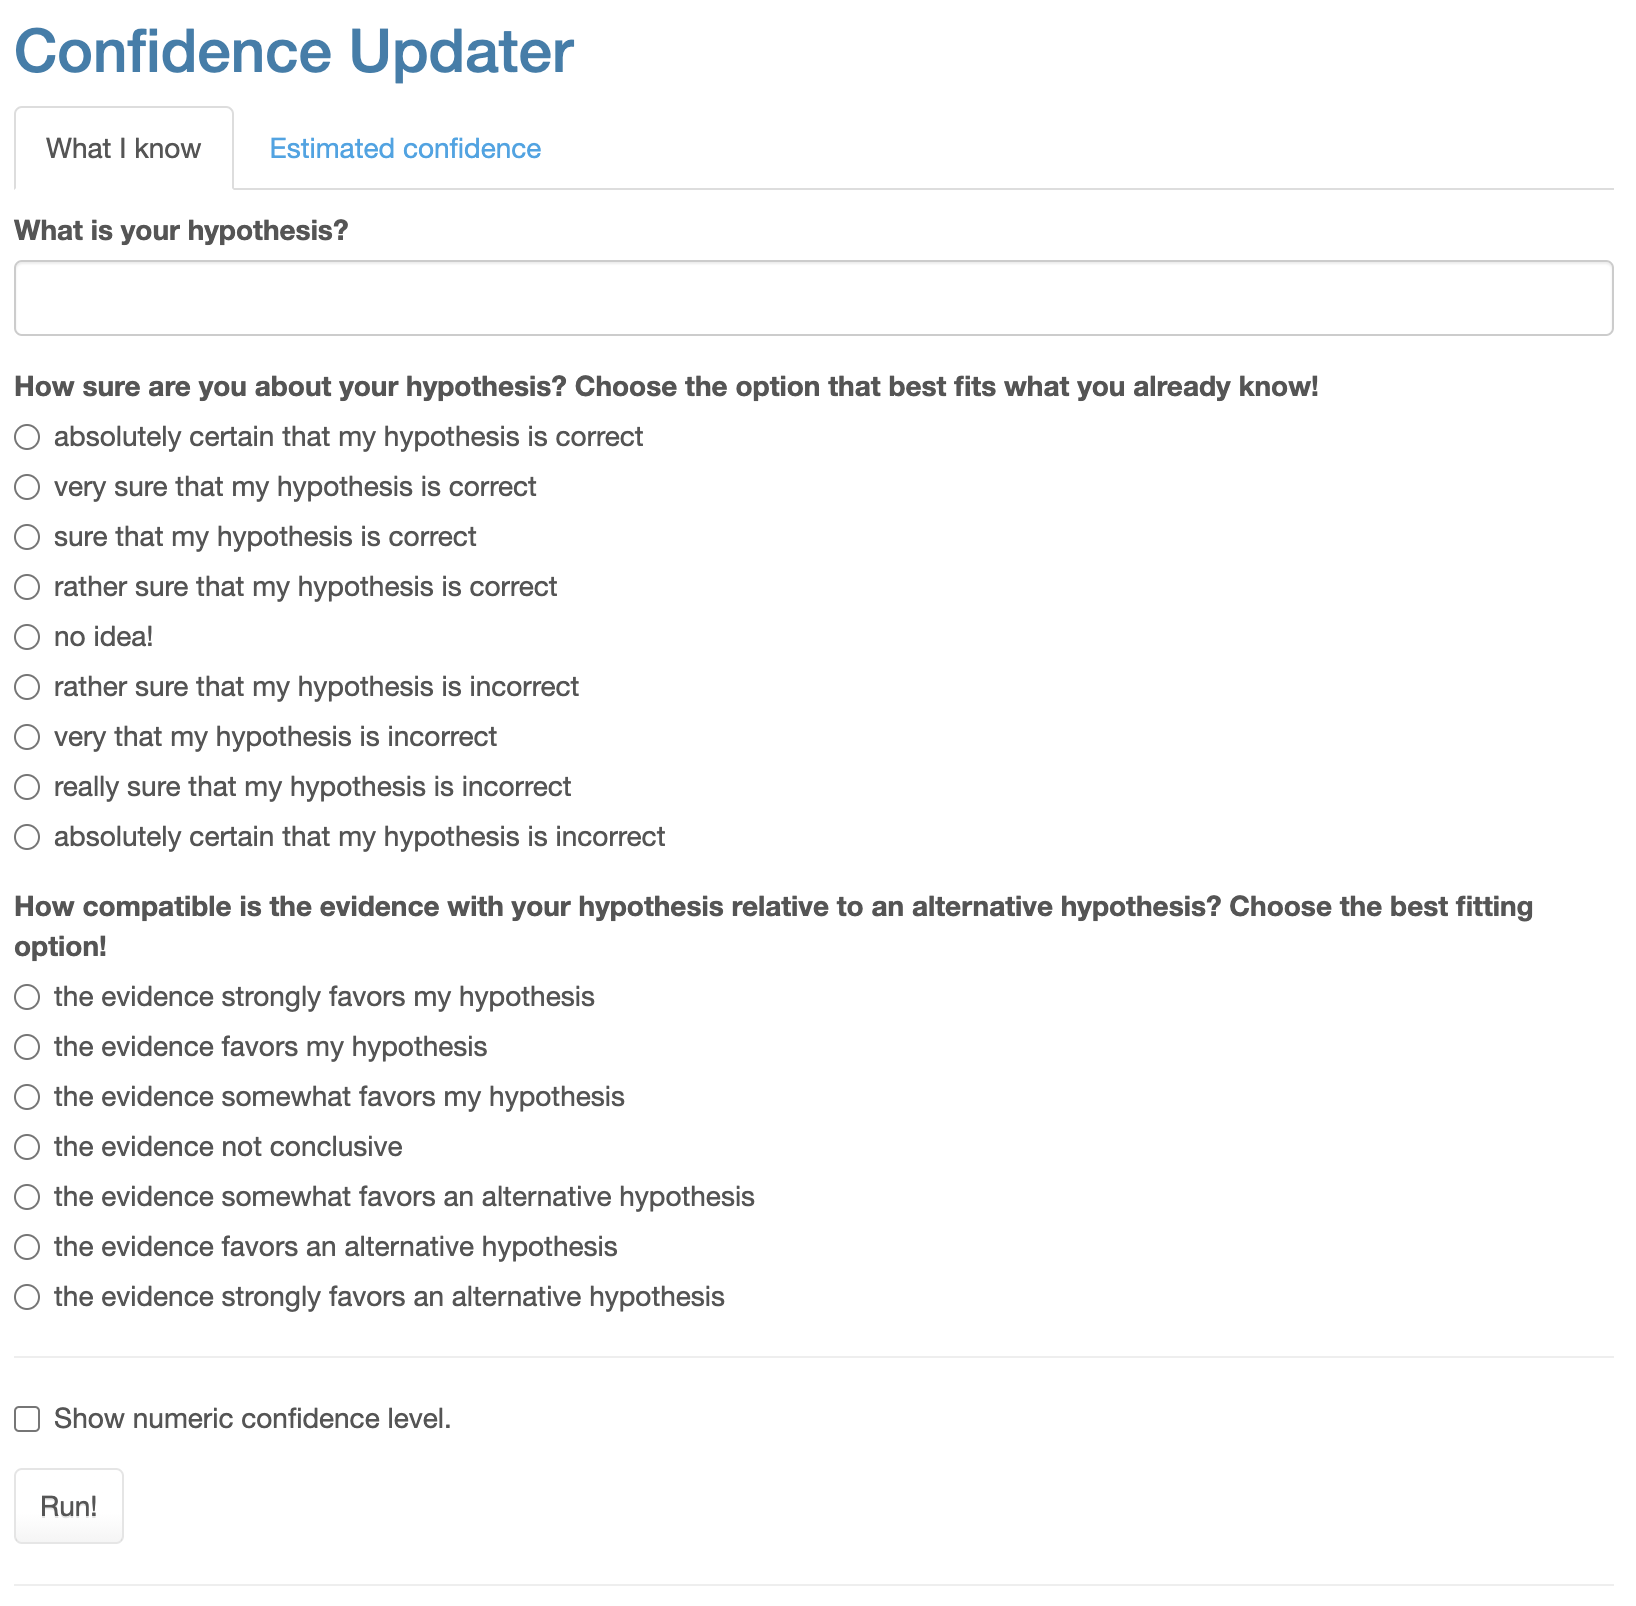
\includegraphics[width = .785\paperwidth]{confidence-updater-input.png}
\caption{Shiny web application for updating one’s confidence in a hypothesis following Bayes' Theorem. $P(H)$ corresponds to the second question (How sure are you about your hypothesis?); \ital{R} corresponds to the second question (How compatible is the evidence with your hypothesis relative to an alternative hypothesis?).}
\label{fig:confidence-updater-input}
\end{center}
\end{figure*}

Using the app, one can obtain an estimate--based on Bayes' Theorem--for the confidence one can have in a hypothesis based upon the degree of one's belief in the initial hypothesis--one's prior--$p(H)$, as well as the predictive updating power of the new evidence, \ital{R}. One can see the example output in Figure~\ref{fig:confidence-updater-output}.

\begin{figure*}[h]
\begin{center}
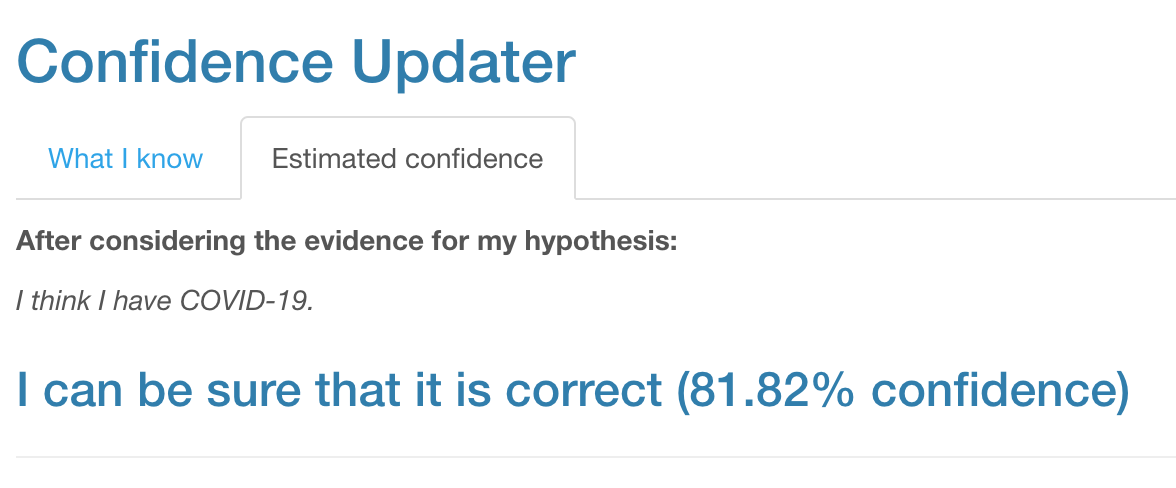
\includegraphics[width = .785\paperwidth]{confidence-updater-output.png}
\caption{Output from the Shiny app}
\label{fig:confidence-updater-output}
\end{center}
\end{figure*}

The principles from the previous section are reflected implicitly and explicitly in the app.

The first principle, \ital{Be open to new evidence}, is emphasized as a natural consequence of Bayes' Theorem and the options \ital{absolutely certain that it is correct} and \ital{absolutely certain that it is incorrect} in the "How sure are you about your hypothesis?" section of the confidence updater. \\ When students select from among these options, $p(H)$ is set to 1 (absolutely certain that it is correct) or 0 (absolutely certain that it is incorrect) respectively. In such cases, neither the tentative (or changeable) nature of scientific knowledge nor the empirical basis of science are manifest, though both are key elements of science \parencite{abd1998nature}.

In consequence, whatever updating factor \ital{R} students choose, the updated confidence will always be the same as the initial hypothesis--the prior--$p(H)$ and the consideration of the new evidence becomes pointless. In other words, in such cases, no amount of data may change one's belief. From this perspective, a question could be considered to be not scientific, as empirical evidence has no bearing on the answer to the question. \\

If students selected any of the options that are equivalent to $p(H)$ = 1, then observe strong contrary evidence, and wonder how this does not affect the updated confidence are observing the evidence, a teacher could refer to principle a) and point out to students how this degree of belief can inhibit changes in beliefs even when confronted with strong evidence--as the students may have just experienced when using the app. \\

As \textcite{warren_quantitative_2018} points out, ``the fact that we can never reach a probability of zero is the quantitative expression of the maxim that we should never rule out any hypothesis with an absolute certainty'' (p. 371). At the same time, even ``in cases where a hypothesis is confirmed by multiple experiments, the posterior probability will approach but never reach, a value of 1; this expresses the maxim that one ought never to have absolute confidence in the truth of a hypothesis.'' (p. 371). In other words, there are no certainties where it comes to Bayesian epistemology. This reflects philosophical and historical accounts of science that emphasize its mutability over time \parencite{Kuhn1962} as expressed in principle 1). \\

The second principle, \itel{account for what is already known} appears in the wording of the prompt for selecting $p(H)$ and becomes visible to students as it effectively moderates the power of the evidence. When prior beliefs and evidence align, the updated confidence is larger in comparison to either having no idea” before or having prior beliefs that do not align. Students could notice this if they compare the updated confidence $p(H|E)$ for students that had the same prior belief but evaluated the evidence differently or had different prior beliefs but evaluated the evidence in the same way. Again, as \textcite{warren_quantitative_2018} points out, “the fact that everyone starts with subjective prior probabilities and yet inevitably converges to a single asymptotic result illustrates the objective aspect of science” (p. 371), which can help build trust in science. \\

Finally, the last principle, \ital{consider alternative explanations} is reflected in how the prompt for \ital{R} is worded. Further, when students use the confidence updater, students should be encouraged to argue for their choice of \ital{R} and be able to explain why they choose a specific option. In such an argument, students following the prompt should not only consider how their evidence supports their own hypothesis but also how compatible it is with alternative hypotheses. That students must select the value for \ital{R}, the predictive updating factor, is notable. Students must figure out the extent to which any single laboratory activity contributes to what we collectively know about a scientific phenomenon: As \textcite{warren_quantitative_2018} writes, it leads to a more realistic view of what laboratory activities can accomplish (i.e., few single introductory physics experiments are likely to overturn established knowledge about the physical world, but they can lead to us updating our understanding)--as well as one that emphasizes scientific sense-making to a greater extent. \\

\subsection{Using the Confidence Updater app}

How does using the confidence updater change a typical science class activity? Here we sketch how using the confidence updater can provide rich opportunities to discuss and reflect on epistemic attitudes. A standard activity at the middle grades levels is to work to understand the relations between amperage, \ital{I}, resistance, \ital{RE}\footnote{We use \ital{RE} for electric resistance--instead of the traditional \ital{R}--to avoid confusion with the updating factor \ital{R}}, and voltage \ital{V}, i.e., \ital{Ohm’s law}, $V=RE*I$. \\

To explore the relations reflected in Ohm's law, students can measure the amperage in a circuit at different voltages, keeping the resistance fixed, or constant. At the beginning of the activity, students can be asked to generate different hypotheses for the relationship between amperage and voltage. In our experience, students often propose a proportional (or linear), inverse, or quadratic relationship for this relationship--when resistance is held constant. Based upon their initial ideas--that the relationship is proportional, inverse, or quadratic, they may test their hypotheses using the app. \\

Specifically, following the second principle, students can now specify their prior confidence in their group’s hypothesis. Students may very well choose different priors based on their individual experiences. Now, they may proceed and record a number of measurements of the current for different voltages and then graph the data. \\

Figure~\ref{fig:example-student-graph} shows an example graph. \\

\begin{figure*}[h]
\begin{center}
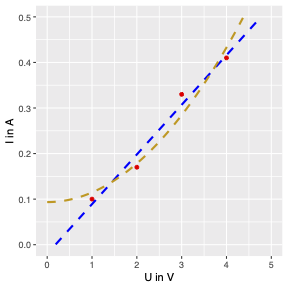
\includegraphics[width = .5\paperwidth]{ohm-graph.png}
\caption{An example student graph}
\label{fig:example-student-graph}
\end{center}
\end{figure*}

When students are asked to evaluate the Evidence and set a value for \ital{R}, they are primed to consider to what extent the evidence is consistent with their hypothesis relative to an alternative hypothesis, reflecting principle 3. Looking at the graph one could see evidence for a proportional relationship as well as a higher-order positive relationship (blue and red dashed line in Figure~\ref{fig:example-student-graph}). \\

Thus, the evidence is barely compatible with an inverse relationship between I and U but supportive of both hypotheses that suggest a positive relationship between the variables. Thus, depending on what hypothesis students choose to investigate, they should select “data favors an alternative hypothesis” for R if their hypothesis is an inverse relationship and select “data somewhat favors my hypothesis” if their hypothesis is proportional or quadratic relationship. \\

The updated confidence for every student will depend on their initial confidence--the prior ($p(H)$)--in their hypothesis and the evaluation of the data which will be different across groups. If students compare their results within groups, they should see how the effect of their initial confidence influences the effect of the evidence. However, if they repeat the activity, i.e., use their updated confidence as a new initial belief and collect more data, they should see how consensus is approached over a few iterations unless anyone choose $p(H) = 0$ or $p(H) = 1$, which points to the importance of principle 1).\\

\subsection{How Can Younger Students Update Their Beliefs in a Bayesian Way?}

It is worth briefly considering whether--and if so, how--younger children may engage in a Bayesian activity like that described above. The work of \textcite{kazak2015bayesian, kazak2018emergent} demonstrates how Bayesian activities can be designed for younger students. For a study with fifth grade (10-11-year-old) students, \textcite{kazak2015bayesian} created a game in which students drew one coin/token from each of two bags. If the colors of the two tokens matched, then students won. The question students were tasked to answer was, "Is the game fair or not?". They played four different rounds of the game (using four different sets of bags). \\

Prior to playing the bag, through a worksheet, students a) articulated whether or not the game was fair and b) their confidence in their beliefs about the fairness of the game. Three of the four games were designed to make the task of determining their fairness challenging. Over the course of playing the games--and using a statistical software tool for learners, TinkerPlots \parencite{konold2005tinkerplots}--students updated both their beliefs about the fairness of the game and their confidence shifted in conjunction with their analysis of data: both generally improved as students collected more data and simulated the collection of data through TinkerPlots. \\

Students first expressed their initial beliefs about the fairness of the game before playing it, updating these beliefs over time. As \textcite{kazak2015bayesian} explained, "since these beliefs can change based on new evidence, it is important to assess the personal degree of confidence in the initial hypothesis or prediction and look at how it changes over the course of gathering new relevant information" (p. 704). This work shows that students can express their \ital{subjective probability} beliefs \parencite[]{batanero2016research,, konold1991understanding} and--critically--update them over time. An instructional implication of this research is that educators can elicit students' ideas about what they think about a phenomenon prior to conducting an investigation (and collecting data). This is an instructional practice already familiar to science educators and science teacher educators \parencite{windschitl2018mbitious, windschitl2012proposing}. \\

In addition to eliciting students' ideas, though, educators can also prompt students to consider how confident they are in their beliefs or ideas. Reflecting upon and "updating" these beliefs can be supported over the course of investigations (and data analyses) by prompting students to consider both their beliefs and confidence over the course of an activity, which can support students to begin to understand the three principles that characterize Bayesian reasoning. \\

\section{Toward a Bayesian Research and Development Agenda in Science Education}

In the last section, we provided an example of how Bayesian principles can be made accessible to a large part of the K-12 science classroom when we use tools like the Confidence Updater app or approaches that prompt students to consider their beliefs and their confidence in them and how they can be modified over time. Based on findings with older students, this work has the potential to support students' epistemic understandings about science \parencite{warren2018quantitative, warren2020impact}. We also have findings from past classroom-based research that "modifying predictions based on previous results appeared to be intuitive for young children" \parencite[, p. 53]{kazak2018emergent}. In this way, beliefs  about the nature of knowing and knowledge-creation could in turn help to build trust in science. But, there are other ways in which a Bayesian perspective could support reasoning about uncertainty and probability more generally. There are several avenues through which this can be approached. \\

First, research on the role of Bayes' in education has mostly been carried out in the context of undergraduate statistics education, in which there have been reviews \parencite{dogucu2021}, recommendations and calls to action \parencite{gpkpwc18, h_a20, dogucu2021}, examples, and design options \parencite{a02, b02,g08, w17, h_j20} and debate \parencite{jrhrr20} over how to advance the place of Bayesian methods in undergraduate statistics and data science degree programs. Why has there been this attention? The accessibility of Bayesian methods in undergraduate classes is the result of advances in the necessary (for many uses) computer power \parencite{gpkpwc18} as well as the availability of tools that facilitate Bayesian analysis, especially for newcomers \parencite{ah20}. As evidenced by the recent special issue of the \emph{Journal of Statistics Education} of which several of the above-referenced articles are part, the pedagogy of Bayesian statistics is an active area of research in statistics education at the undergraduate level. \\

Despite attention from statistics educators and statistics education researchers, there has been little research outside of statistics education in the broader science education community. Two publications merit mention, though. The work of \textcite{so12} and \textcite{n11} both applied Bayesian perspectives to the science practice of argumentation. Szu and Osborne presented the case for how and why Bayes' Theorem can apply to research and practice on scientific reasoning, broadly, and argumentation, particularly. This paper represents the most comprehensive account of the relevance of Bayesian methods for science education. Szu and Osborne argue that Bayes' is useful as both a formal mathematical tool and a conceptual one; indeed, they write that considering the degrees of certainty in beliefs that individual students hold—different from applications of Bayes' Theorem that follow more or less deterministically from ``external, objectively probabilistic systems'' (p. 61)—is ``the key leap that characterizes the debate about the value of Bayesian inference as a model of scientific reasoning'' (p. 61). In this way, Szu and Osborne argue that the greatest use of Bayes' Theorem in science classrooms is as a model of informal scientific reasoning, aligning with similar (informal) approaches to inference within the statistics education research community \parencite{batanero2016research, mr18}. They offer some research-related backing for the use of Bayes' Theorem (e.g., noting how conceptual change research, particularly, and constructivist research, broadly, can both be explained coherently within a Bayesian approach) as well as some practical, instructional recommendations, some of which we detail later in this section. \\

\textcite{n11} work on Bayesian approaches to argumentation describes both an application of Bayesian methods in K-12 classroom contexts and ideas about how Bayesian methods can serve as an analytic framework for students’ argumentation. Concerning the latter, Nussbaum describes how the social issue of raising taxes to provide resources to homeless individuals was a rich context for students to engage in forms of Bayesian reasoning. In this application, Nussbaum describes how the prior and likelihood could be obtained from empirical evidence—in this way, illustrating what \textcite{so12} characterize as the more externally objective use of Bayes' Theorem—and how the estimates that result from applying Bayes' Theorem led students to re-evaluate their initial arguments. \\

The work of \textcite{so12} and \textcite{n11} begin to apply Bayesian ideas to science education and other relevant classroom contexts, making Bayesian ideas more vivid in the process. Neither, though, speaks to how a Bayesian perspective could have a role in bolstering understanding or trust in science by learners and others. More generally, these two contributions are steps toward conceiving what a Bayesian perspective may offer science education, but there remains room to build further. For instance, despite their association with statistical methods that are growing in use in post-secondary contexts and in industry \parencite{mcgrayne2011theory}, no science education scholarship has applied Bayesian methods to another science practice, that of analyzing and interpreting data. In this way, being clear about what we mean by a \ital{Bayesian perspective} is important: this perspective could be associated not only with a \ital{practice} (analyzing data) but also as a cross-cutting concept \parencite{nrc12} that can, in the context of learning about particular scientific ideas, unite the practice of argumentation with analyzing and interpreting data with the notions of probability and (un)certainty. Bayesian methods can also provide a framework that includes a set of epistemological principles and a partial explanation for the process of how and why people change their ideas in light of new information or data--two key components of (and potential barriers to) how members of the public understand and act upon scientific knowledge \parencite{sinatra2014addressing}.

\section{Conclusion}

In light of how scientific knowledge can be presented to learners as immutable \parencite{d90, manz2018supporting, carey1993understanding}, it may be unsurprising that learners--and people--are dismayed when scientific knowledge that was once considered to be the consensus is modified or even nullified. When learners do not have a way to think about uncertainty, they may adopt an approach that considers scientific knowledge to be correct or incorrect--or for scientific sources to provide evidence that is true or false. From a Bayesian perspective, uncertainty about scientific knowledge can be viewed in terms of the degrees of belief that a person holds toward a belief, claim, or research--any prior information--in light of new evidence. We conjecture in this paper that such a paper can bolster individuals' trust in science by providing a principled, flexible way to reason about uncertainty.

Indeed, a key potential benefit of Bayes' may be that it provides a framework for helping students to transition from their conceptual understanding of scientific ideas to quantitatively analyzing data. In this way, we argue for the use of a Bayesian perspective that could influence research about (and teaching to support) learners' epistemic considerations and how learners' ideas change over time--factors that may have a bearing on how they understand science outside of school, or later as adults \parencite{sinatra2014addressing}. Thus, we see there is a number of ways in which a Bayesian perspective can influence science education--and, therefore, we see  a number of mechanisms through which Bayesian methods could bolster trust in science, from specific teaching approaches, such as those that could be constructed around the Confidence Updater widget \parencite[]{warren_impact_2020, warren_quantitative_2018}, to approaches tailored to younger children \parencite[e.g., ]{kazak2015bayesian, kazak2018emergent}. Somewhat different from the past research focused on the connection between scientific argumentation and Bayes' Theorem \parencite[]{n11, so12}, our aim with this paper was to highlight the broad potential of a Bayesian perspective for reasoning about uncertainty in data and evidence and to offer a few directions for how the potential of Bayes' in future research. \\

Even at a time in which science has made and continues to make great advances, the history of science suggests that uncertainty will not be removed (or even reduced) given scientific progress \parencite{fara2010science}; looking ahead, being able to effectively navigate, counsel, and act in the midst of uncertainty may be as important as it has been at other uncertain points in history. Like the surprising utility of a Bayesian perspective in domains that are similar to education (e.g., developmental science), might an unexpected feature of a Bayesian perspective be that embracing uncertainty--equipped with the tools that Bayesian methods provide--makes individuals and societies more confident? In short, can we build trust in science by embracing uncertainty? We think that these are questions that are \ital{likely} to yield positive results for science educators and those advocating for a more scientifically-informed citizenry and science learners. \\

\printbibliography

\newpage

\section{Appendix A: The Epistemological Axioms that Follow from Bayes' Theorem}

\subsection{Integrating Inductive and Deductive Reasoning With the Bayesian Learning Cycle}

Several years ago, physicists reported that they had observed elementary particles moving faster than the speed of light \parencite{b11}--thus defying Einstein’s theory of relativity. However, instead of celebrating a historic discovery, the scientists started to look for what had gone wrong in their observations. With nearly a century of accumulated evidence that the theory of relativity holds, from a Bayesian perspective, scientists had a very strong prior belief about the speed of light. To change this belief, extraordinary evidence would have been required. Thus, a single instance of apparently faster-than-light elementary particles does not give a likelihood strong enough to change the prior in a meaningful way, and in consequence, the posterior--the knowledge about the world after making an observation--does not change in a meaningful way. \\

Rather than changing their belief about the speed of light, scientists looked for things that could have gone wrong with the measurement. This example shows how a qualitative take on Bayes'’ theorem can explain and predict many aspects of how animals \parencite{o13}, people \parencite{tgk06}, and organizations \parencite{kaj12} learn from observations. Recently, advances in computational power and techniques have started the more and more widespread application of this principle in a quantitative way that allows researchers to precisely express their knowledge about the world and then learn from observations. \\

Expressed in the Bayesian learning cycle (Figure \ref{fig:The Bayesian Learning Cycle}), a Bayesian reasoning framework allows scientists to integrate the strengths of both, inductive and deductive research approaches, in a formalized way. Further, when specifying the prior, scientists openly and explicitly need to describe the uncertainty in the current state of knowledge, and the posterior captures how the data has changed the knowledge and the uncertainty in that knowledge. Thus, Bayesian reasoning is--in principle--open and transparent by design. \\

\begin{figure*}[h]
\begin{center}
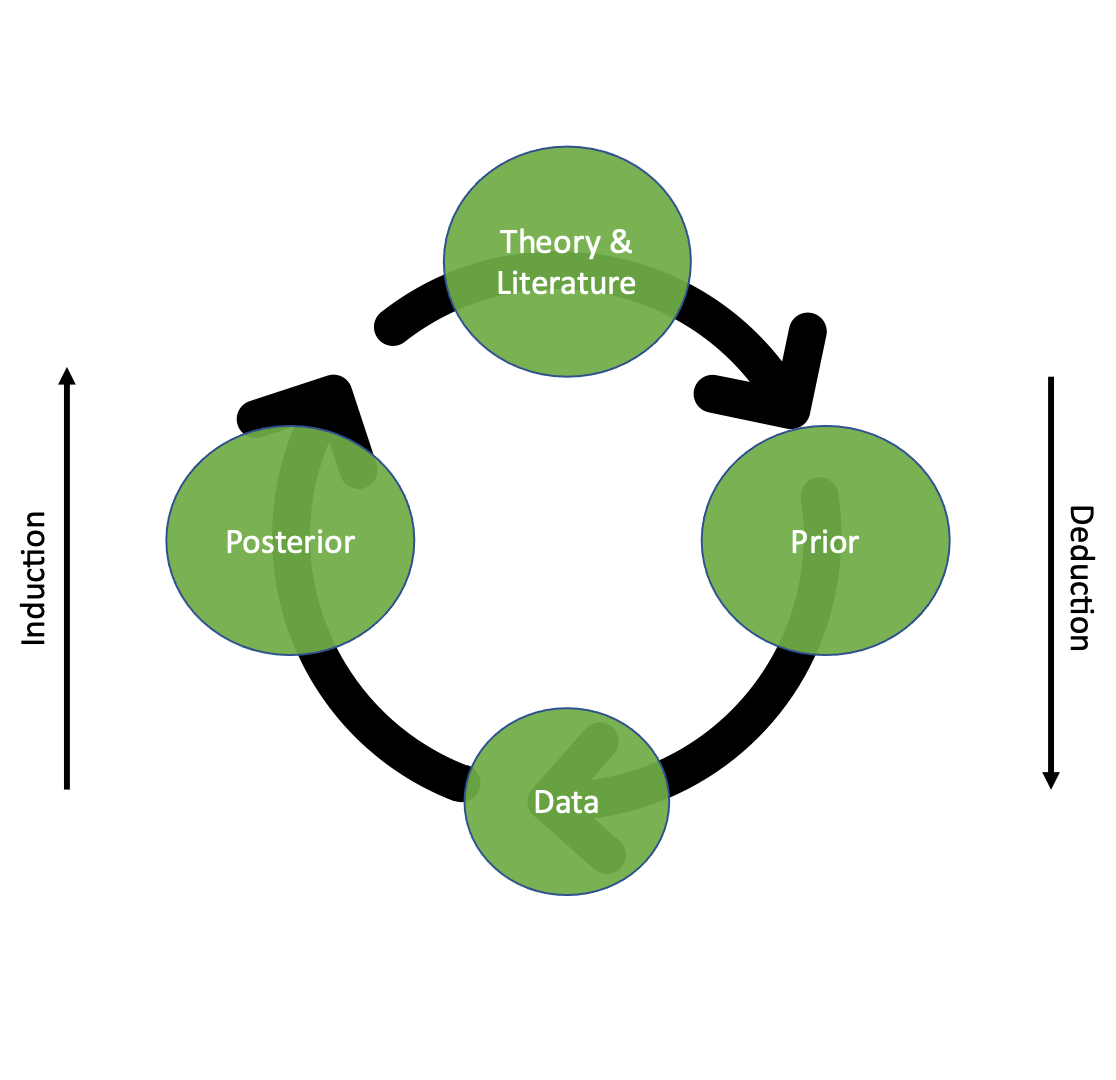
\includegraphics[width = .65\paperwidth]{learning.png}
\caption{The Bayesian learning cycle is a reasoning framework that allows scientists, citizens, and learners to integrate the strengths of inductive and deductive reasoning while making sense of data in light of prior beliefs.}
\label{fig:The Bayesian Learning Cycle}
\end{center}
\end{figure*}

\subsection{Mathematical Axioms That Follow From Bayes' Theorem}

In this section, we build on the idea of the Bayesian Learning Cycle--that a Bayesian perspective aligns with a way of systematically taking in new information to improve what one knows (and how certain one is about what one knows--to elaborate on some general principles related to the nature of knowledge and knowing, or epistemological principles. We illustrate these to later show how they can have a role in the science classroom and how they can be used by individuals outside of classrooms and schools to understand and act upon scientific information. \\

In the previous section, we emphasized the idea that hypotheses, or ideas, gain credibility when they predict the data well, and lose credibility when they predict new data poorly \parencite{WagenmakersEtAl2016CD}. This idea generalizes to the ``Fundamental Inductive Pattern'':
\begin{quotation}

\noindent ``This inductive pattern says nothing surprising. On the contrary, it expresses a belief which no reasonable person seems to doubt: \emph{The verification of a consequence renders a conjecture more credible}. With a little attention, we can observe countless reasonings in everyday life, in the law courts, in science, etc., which appear to confirm to our pattern.'' \parencite[pp. 4-5]{Polya1954Vol2}
\end{quotation}

The rule from Equation~\ref{eq:BayesRule} includes the constant term $p(\text{data})$, which does not involve $\theta$. As a result, Bayes' rule can be re-written as:
\begin{equation}
\label{eq:BayesRulePropto}
p(\theta \mid \text{data}) \propto p(\text{data} \mid \theta) \times p(\theta),
\end{equation}
where `$\propto$' stands for `is proportional to'. Thus, Bayes' rule states that our posterior knowledge $p(\theta \given \text{data})$ is proportional to the likelihood $p(\text{data} \given \theta)$ (or the extent to which the observed data are expected given $\theta$) multiplied by our prior knowledge $p(\theta)$. \\

Equation~\ref{eq:BayesRulePropto} emphasizes that the posterior uncertainty about $\theta$ is a \emph{compromise} between our prior uncertainty about $\theta$ and the predictive performance of $\theta$. But, the posterior uncertainty after having observed the first datum becomes the prior uncertainty for the next datum--and any other data (cf. Figure~\ref{fig:WindowsMacSequential}). Consequently, after having observed another datum, the posterior uncertainty represents a compromise of a compromise. As the data accumulate, the posterior uncertainty is more and more determined by predictive performance, and the impact of the initial uncertainty about $\theta$ is increasingly watered down: `the data overwhelm the prior' \parencite{WrinchJeffreys1919}. \\

This implies (but does not dictate, as we discuss next) that a constant stream of accumulating data ought to bring any two people into an arbitrarily close agreement, no matter how divergent their opinions may have been at the outset. Two caveats exist. First and foremost, the data only overwhelm the prior if that prior is neither equal to zero (denoting an impossibility) nor one (denoting absolute certainty). If someone already knows for certain that a hypothesis is true or false, then you cannot adjust your opinion in light of the data: your initial opinion will be your final opinion, no matter what the data may indicate. Philosophically, adopting such priors is a dangerous practice; for instance, in antiquity, the adage of the \emph{New Academy} --a school of skeptics headed by Carneades-- was ``never assert absolutely''. In modern times, Lindley popularized this idea in statistics and coined it ``Cromwell's rule'' \parencite[p. 104]{Lindley1985}. \\

The second caveat is that, in real life, the data are sometimes relatively slow to overwhelm the prior, as people can be reluctant to change their beliefs (for a Bayesian model see \cite{Gershman2019}). A more extreme case is \emph{belief polarization}: confronted with the same stream of information, two people who hold different opinions may drift further apart instead of moving closer together (but see \cite{Anglin2019}). This appears irrational, but several Bayesian accounts have been offered to explain the phenomenon (e.g., \cite{CookLewandowsky2016,JernEtAl2014}). \\

Next, consider two specific values for $\theta$, $\theta_1$ and $\theta_2$. We can use Bayes' rule to obtain the posterior probability for each one:
\begin{align}
p(\theta_1 \mid \text{data})& =  \frac{p(\text{data} \mid \theta_1) \times p(\theta_1)}{p(\text{data})}\\
p(\theta_2 \mid \text{data})& =  \frac{p(\text{data} \mid \theta_2) \times p(\theta_2)}{p(\text{data})}.
\end{align}
When we divide the posterior probabilities, the common term, $p(\text{data})$, can be dropped from each side of the equation, and we have:
\begin{equation}
    \frac{p(\theta_1 \mid \text{data})}{p(\theta_2 \mid \text{data})} = \frac{p(\theta_1)}{p(\theta_2)} \, \times \, \frac{p(\text{data} \mid \theta_1)}{p(\text{data} \mid \theta_2)}.
\end{equation}
We replace $\theta_2$ with $\mathcal{H}_1$ (i.e., the alternative hypothesis, in which a test-relevant parameter $\xi$ is free to vary) and $\theta_1$ with $\mathcal{H}_0$ (i.e., the null hypothesis in which $\xi$ takes on a fixed value, for instance $\xi=0$):
\begin{equation}
    \frac{p(\mathcal{H}_1 \mid \text{data})}{p(\mathcal{H}_0 \mid \text{data})} = \frac{p(\mathcal{H}_1)}{p(\mathcal{H}_0)} \, \times \, \frac{p(\text{data} \mid \mathcal{H}_1)}{p(\text{data} \mid \mathcal{H}_0)}.
\end{equation}
This way of writing Bayes' rule highlights that extraordinary claims require extraordinary evidence -- if a particular hypothesis $\mathcal{H}_1$ is extremely unlikely a priori, the prior odds $\frac{p(\mathcal{H}_1)}{p(\mathcal{H}_0)}$ are stacked against it, and for the posterior odds to favor $\mathcal{H}_1$ the support from the data (i.e, the degree to which $\mathcal{H}_1$ predicts $\mathcal{H}_0$) needs to be overwhelmingly strong. \\  

Bayes' rule can also be shown to embody the \emph{principle of parsimony}: the rule implicitly contains a preference for the simplest model that explains the data well. To see this, consider a coin with two sides and let parameter $\xi$ indicate the chance that the coin lands heads on any throw. The null hypothesis holds that the coin is fair, with heads and tails equally likely: $\mathcal{H}_0: \xi = \nicefrac{1}{2}$. The alternative hypothesis that we entertain here specifies that the coin may be any of the following options with equivalent likelihood: double-tails, fair, or double-heads, $\mathcal{H}_1: \xi \in \{0, \nicefrac{1}{2}, 1\}$. \\

The coin is tossed and heads is observed. The probability of this datum is \nicefrac{1}{2} under $\mathcal{H}_0$; under $\mathcal{H}_1$, it is $p(\text{heads} \given \xi=0) \cdot p(\xi=0 \given \mathcal{H}_1) + p(\text{heads} \given \xi=\nicefrac{1}{2}) \cdot p(\xi=\nicefrac{1}{2} \given \mathcal{H}_1) + p(\text{heads} \given \xi=1) \cdot p(\xi=1 \given \mathcal{H}_1) = 0 \cdot \nicefrac{1}{3}  + \nicefrac{1}{2} \cdot \nicefrac{1}{3} + 1 \cdot \nicefrac{1}{3} = \nicefrac{1}{2}$. So, the datum is equally likely under $\mathcal{H}_0$ and $\mathcal{H}_1$: both models receive an equal amount of support. This means the first outcome does not change our conviction concerning $\mathcal{H}_0$ versus $\mathcal{H}_1$. The datum did, however, change our beliefs about $\xi$ under $\mathcal{H}_1$. Specifically, we now know that $\xi$ cannot be zero; moreover, the datum was twice as likely under $\xi=1$ as under $\xi = \nicefrac{1}{2}$, so that our posterior distribution for $\xi$ under $\mathcal{H}_1$ is now $p(\xi = \nicefrac{1}{2}) = \nicefrac{1}{3}, p(\xi = 1) = \nicefrac{2}{3}$. \\

The coin is tossed a second time and it lands tails. Under $\mathcal{H}_0$, the probability of this happening is again $\nicefrac{1}{2}$, so the total probability for the data sequence $\{\text{heads}, \text{tails}\}$ under $\mathcal{H}_0$ equals $\nicefrac{1}{2} \cdot \nicefrac{1}{2} = \nicefrac{1}{4}$. Under $\mathcal{H}_1$, the probability of the second toss landing heads is computed under the posterior distribution obtained after the first toss, and this yields: $p(\text{tails} \given \xi = \nicefrac{1}{2}) \cdot p(\xi=\nicefrac{1}{2} \given \mathcal{H}_1) + p(\text{tails} \given \xi = 1) \cdot p(\xi=1 \given \mathcal{H}_1) = \nicefrac{1}{2} \cdot \nicefrac{1}{3} + 0 \cdot \nicefrac{2}{3} = \nicefrac{1}{6}$. The total probability for the data sequence $\{\text{heads}, \text{tails}\}$ under $\mathcal{H}_1$ equals $\nicefrac{1}{2} \cdot \nicefrac{1}{6} = \nicefrac{1}{12}$. This means that the observed data provided $(\nicefrac{1}{4}) / (\nicefrac{1}{12}) = 3$ times more support for $\mathcal{H}_0$ than for $\mathcal{H}_1$. This happens because $\mathcal{H}_1$ "spreads out" its predictions, hedging its bets. In contrast, the simple model $\mathcal{H}_0$ made a precise prediction. \\

Instead of learning about the predictive performance one observation at a time of $\mathcal{H}_0$ and $\mathcal{H}_1$, we could also have considered the probability that the models assign to the entire sequence $\{\text{heads}, \text{tails}\}$. Under $\mathcal{H}_0$ we again have $\nicefrac{1}{2} \cdot \nicefrac{1}{2} = \nicefrac{1}{4}$. Under $\mathcal{H}_1$, we notice that the data falsify both $\xi=0$ and $\xi=1$. This leaves $\xi=\nicefrac{1}{2}$, which suggests the same answer as under $\mathcal{H}_0$, that is $\nicefrac{1}{2} \cdot \nicefrac{1}{2} = \nicefrac{1}{4}$. However, we need to multiply this probability with $\nicefrac{1}{3}$, the prior probability that $\xi=\nicefrac{1}{2}$. This is the penalty for complexity that $\mathcal{H}_1$ pays for entertaining three different values of $\xi$ from the outset. Thus, in addition to reflecting the principle of parsimony and highlighting the utility of parsimonious explanations, Bayes' rule includes a automatic ``Ockham's razor'' \parencite{Jeffreys1939,JefferysBerger1992} in the sense that daring predictions are rewarded when they come true. \\
 
Lastly, we can also write Bayes' rule as follows:
\begin{equation}
\begin{split}
    p(\mathcal{H}_1 \mid \text{data})& = \frac{p(\text{data} \mid \mathcal{H}_1) p(\mathcal{H}_1)}{p(\text{data})}\\
    & = \frac{p(\text{data} \mid \mathcal{H}_1) p(\mathcal{H}_1)}{p(\text{data} \mid \mathcal{H}_1) p(\mathcal{H}_1) + p(\text{data} \mid \mathcal{H}_0) p(\mathcal{H}_0)}.
\end{split}
\end{equation}
This equation shows that the posterior plausibility is dictated by the predictive performance for $\mathcal{H}_1$ and $\mathcal{H}_0$, weighted by the prior plausibility of each hypothesis. In other words, ``The Bayesian world is a comparative world in which there are no absolutes.'' \parencite[p. 308]{Lindley2000}. This is in stark contrast to $p$-value statistical hypothesis testing, in which a statistical model (the null hypothesis) is judged in isolation. \\ 

\end{document}
